\documentclass[11pt]{article}
\pagestyle{myheadings}
\markright{Pythia-Trento Jet Study and Date - \today}
\usepackage{graphicx}
\usepackage{color}
\usepackage{enumitem}
\usepackage{hyperref}
\usepackage{amsmath}
\usepackage{pdfpages}
\usepackage[nottoc,numbib]{tocbibind} %inserts References in table of contents
\usepackage[sort&compress]{natbib}
%
\textwidth 7.0in
\textheight 9in
%\itemsep 0pt
\parsep 5pt
\parindent 10pt
\parskip 5pt
\hoffset -1.in
\voffset -0.5in

\begin{document}

%
% Useful command to condense itemize lists
%
\newcommand{\zapspace}{\topsep=1pt\partopsep=1pt\itemsep=1pt\parskip=2pt}
\newcommand{\trento}{\mbox{T$_{\rm R}$ENTo}}

\begin{center}
{\Large \bf Pythia Jet Finding Study with Trento Backgrounds\\}
\bigskip
Joseph Simpson and Ron Soltz
\end{center}

\begin{abstract}
We present results applying the Pythia SlowJet Finder to Pythia generated QCD and QED hard processes in the presence of simulated heavy ion backgrounds.  The hard process events are generated with Pythia version~8.219 for $\sqrt{s}$200~GeV proton-proton collisions and the backgrounds are generated by the Reduced Thickness Event-by-event Nuclear Topology model \trento\ for Au-Au collisions with a nucleon-nucleon cross-section of 4.23~fm$^2$.  The \trento\ model is used to determine the initial entropy and ellipticity from which the total charged particle multiplicity and elliptic flow are determined.  We report results in the form of event displays, total $p_T$ distributions, and fragmentation distributions for SlowJet applied to Pythia events with and without the simulated heavy ion backgrounds.
\end{abstract}

\tableofcontents

\newpage 

\section{Introduction}
\subsection*{Motivation}

The study of jet-quenching in heavy ion collisions, how jets lose energy as they evolve within the quark-gluon plasma (QGP) is one of the most important topics remaining in the quest to understand the detailed properties of the QGP.  However, the task of reconstructing jets within a high multiplicity heavy ion background can be difficult.  Fluctuations in the background can be falsely reconstructed as jets, and true jets that lose energy in the plasma can easily be buried within the backgrounds.  The purpose of this study is to develop a set of simple tools to study jets within an environment that simulates the basic elements of a heavy ion background with thermal particle production and radial and elliptic flow, and then to use these tools to create visual images of the jets and quantitative distributions of jet properties in a fluctuating heavy ion background.  For this study, it is assumed that the identity, mass, and momenta of all produced particles are precisely known.  We do not attempt to include any detector effects.

\subsection*{Software Framework}

For this study we work with the Pythia 8.219 Python package, which can be called from Python 2.7.  We use the SlowJet routines that are included in the Pythia installation.  SlowJet provides an {\it anti-k$T$} jet-finding algorithm that produces identical results to FastJet, but does not run as quickly.  Most of the analysis is done using numpy and matplotlib.pyplot packages.  The \trento\ version 1.3 code is run as a stand-alone program.  \trento\ outputs are saved to text files and read from Python scripts, although it is also possible for it to be called directly from within Python.  Unless stated otherwise, all \trento\ backgrounds are for minimum bias distributions.  Additional details on using these packages are given in the descriptions below.

\section{Running Pythia}
%
%Describe pythia settings, show lego plot of jet events, for QCD and QED
%Show distribution of jet pT distributions for QCD and QED
%
Pythia allows users to set the beam center-of-mass energy ($E_{CM}$). By default Pythia sets $E_{CM}$ to 14 TeV, the default for all our programs is 200 GeV.  Initial QCD or QED hard scattering processes may be turned on or off. Pythia also allows restrictions to be set on the transverse momentum produced by hard scattering ($p_{THat}$ or jet $p_T$). For our programs the jet $p_T$ range is typically 20-25 GeV. Figure 1 shows the distribution of jet $p_T$ for both various QCD and various QED processes restricted to the range of 20-50 GeV. The upper histogram of figure 1 shows the four most common QCD hard processes produced by Pythia. The different processes are shown in the legend. Gluons are represented by "g", quarks (uds) are represented by "q", and anti-quarks (uds) are represented by "q(bar)." There are also other hard processes, such as those that involve heavy quarks, but they occur so infrequently that they are not included. The lower histogram shows all five of the QED hard processes, however only two of the processes occur frequently. For these processes photons are represented by "gamma," and fermions participating in electroweak interactions are represented by "f" and "f(bar)."

Figure 2 shows two lego plots, one for a QCD event and one for a QED event. These plots demonstrate how our programs are able to display each Pythia event. Each particle that is produced from a Pythia event is binned in a 2 dimensional histogram depending on its pseudo-rapidity ($\eta$) and azimuthal angle ($\phi$). The histogram bins are weighted by transverse energy ($E_T$). In both plots it is easy to identify the jets produced by the Pythia events. For the QED plot it is important to note that one of the jets is produced by only a single photon. 

\begin{figure}[h]
\begin{center}
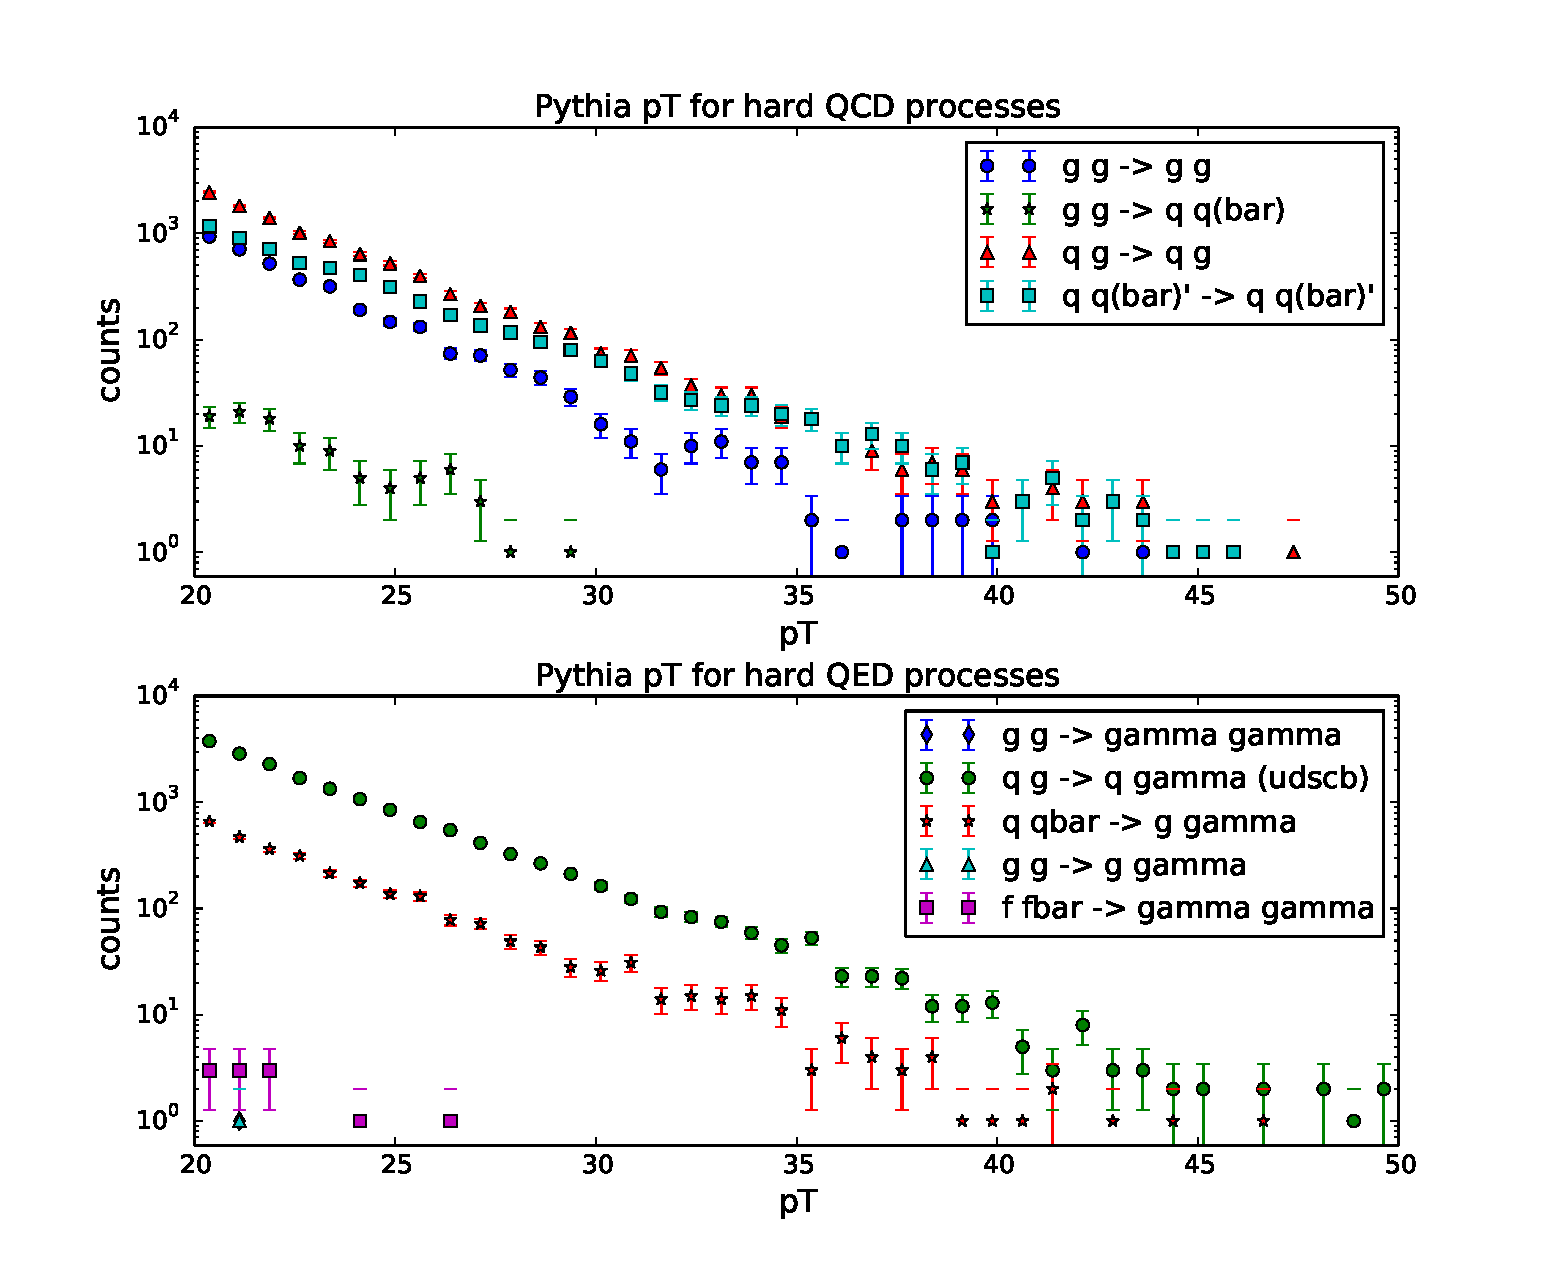
\includegraphics[width=0.8\textwidth]{pT_pythiaEvents.pdf}
\label{fig_label}
\caption{Distribution of jet pT for QCD and QED processes for 20,000 events.  Figure created with [python pT\_pythiaEvents.py -m 20000]}
\end{center}
\end{figure}

\begin{figure}[h]
\begin{center}
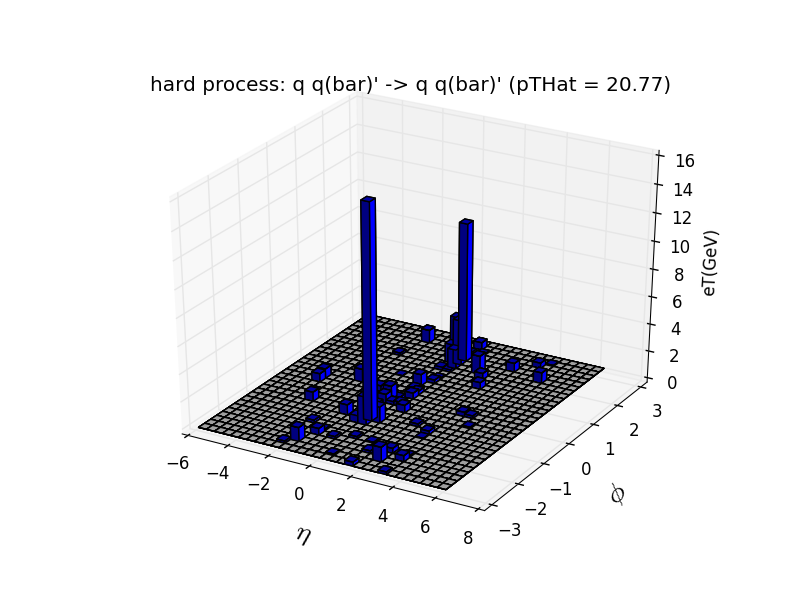
\includegraphics[width=0.49\textwidth]{2d_hist_jetplot.png}
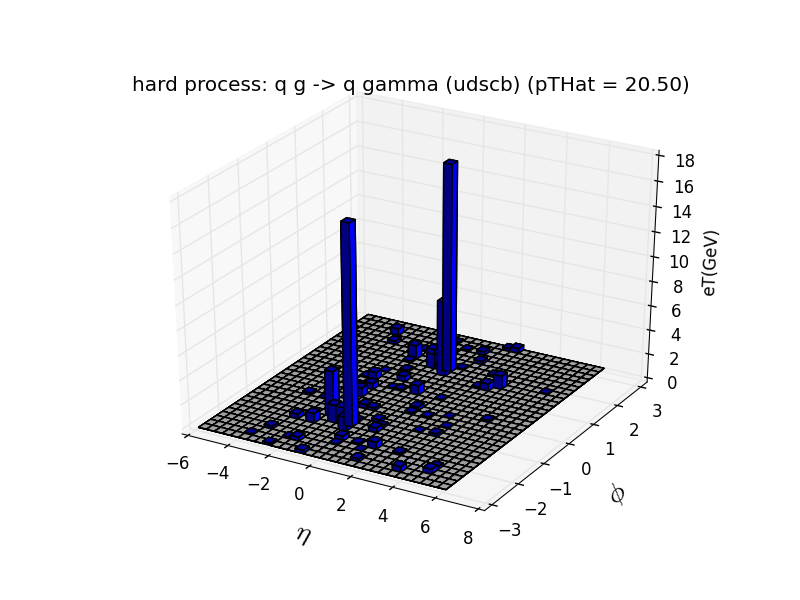
\includegraphics[width=0.49\textwidth]{2d_hist_jetplot2.png}
\label{fig_label}
\caption{Pythia event display for a QCD event, shown to the left, and a QED event shown to the right.  Left figure created with [python 2d\_hist\_jetplot\_wcol.py -o -b 30]. Right figure created with [python 2d\_hist\_jetplot\_wcol.py -o -c -q -b 30]}
\end{center}
\end{figure}

\section{Adding Trento Backgrounds}
%
% Describe how Trento is run, list parameters.
% Describe how we convert Trento output into particle number
% Explain how we generate pT, eta, and phi.
% Explain we add radial flow and elliptic flow from epsilon_2 variable.
%
\trento\ allows users to input several physical options in order to create realistic heavy ion collision backgrounds. These options include two projectiles, number of events, reduced-thickness, fluctuation, nucleon-width, cross-section, and a normalization factor. For each data set,  we used non-deformed gold (Au) nuclei with 197 nucleons each. We produced 100,000 events for several different cross-sections. All other physical options were left to their default settings: reduced-thickness = 0, fluctuation = 1, nucleon-width = 0.5 fm, and normalization = 1. Different cross-sections correspond to different beam $E_{CM}$ per nucleon pair. The cross-sections (in units of fm$^2$) that we used to simulate the different beam energies are shown in table 1. \trento\ reads in the options and produces a text file listing several event properties for each event: event number, impact parameter, number of participants, initial entropy, and properties of flow. The produced \trento\ text files were then imported into our programs as an array of event data.

\begin{center}
\begin{table}
\centering
\caption{Cross sections as a function of $\sqrt{s_{nn}}$}
\begin{tabular}{|c|l|}
\hline
$E_{CM}$(GeV)& $\sigma_{nn}$(fm$^2$) \\
\hline
200 & 4.23 \\
\hline
130 & 3.96 \\
\hline
62.4 & 3.60 \\
\hline
39 & 3.43 \\
\hline
27 & 3.32 \\
\hline
19.6 & 3.25 \\
\hline
15.0 & 3.20 \\
\hline
7.7 & 3.12 \\
\hline
\end{tabular}
\label{}
\end{table}
\end{center}

To use the \trento\ data as we intended we had to produce accurate Au-Au multiplicities for the various beam energies. To do this we fit the \trento\ data to PHENIX data. We created a histogram for the number of participants in each \trento\ event and weighted the bins by the initial entropy. We then scaled the \trento\ data at each energy by a constant to fit it to the PHENIX data of charged multiplicity vs. number of participants. The fit and the produced plot is shown in figure 3. The \trento\ data points are the open shapes that are connected by lines. Using the constants from the fit at each energy allowed us to create multiplicity values from the initial entropy values. The constant for the 200 GeV data was 4.65905256.

Using the \trento\ multiplicity values we now knew how many background particles to create for each \trento\ event. To generate values of transverse momentum ($p_T$), pseudo-rapidity ($\eta$), and azimuthal angle ($\phi$) for each particle we used the numpy random number generator. For $\phi$  and $\eta$ we created flat distributions between -$\pi$ to $\pi$ and -2 to 2, and for $p_T$ we sampled from a Gaussian deviate, which is equivalent to a thermal Boltzmann distribution. We also included radial and elliptic flow into our background distributions by using the $\epsilon_2$ variable from the \trento\ data. First we calculated the initial transverse rapidity ($y_T$) and then applied flow as an additive boost. 
\[y_{Boost} = \rho \times \rho_0 + \rho_2 \times \epsilon_2 \times cos(2\phi)\]
The scaling parameter for radial flow ($\rho_0$) that we used was 0.85 from Retiere and Lisa, PRC70.044907 (2004), table 2.  The scaling parameter for elliptic flow ($\rho_2$) was 0.15 from Alver and Roland, PRC81,054905 (2010), fig 4. Again using the numpy random number generator we created a normalized radial distance ($\rho$). After applying flow, $y_T$ was converted back to $p_T$. The mass used for these calculations was chosen randomly from one of nine different particles that were included in the produced background. These particles consisted of pions, kaons, protons, and neutrons, as well as their anti particle counterparts. Figure 4 shows the background display produced from \trento\ events. Again each particle that is produced is binned in a 2 dimensional histogram in ($\eta$,$\phi$) space. For this plot the histogram bins are weighted by $p_T$. There are no jets produced within the \trento\ background.

\begin{figure}[h]
\begin{center}
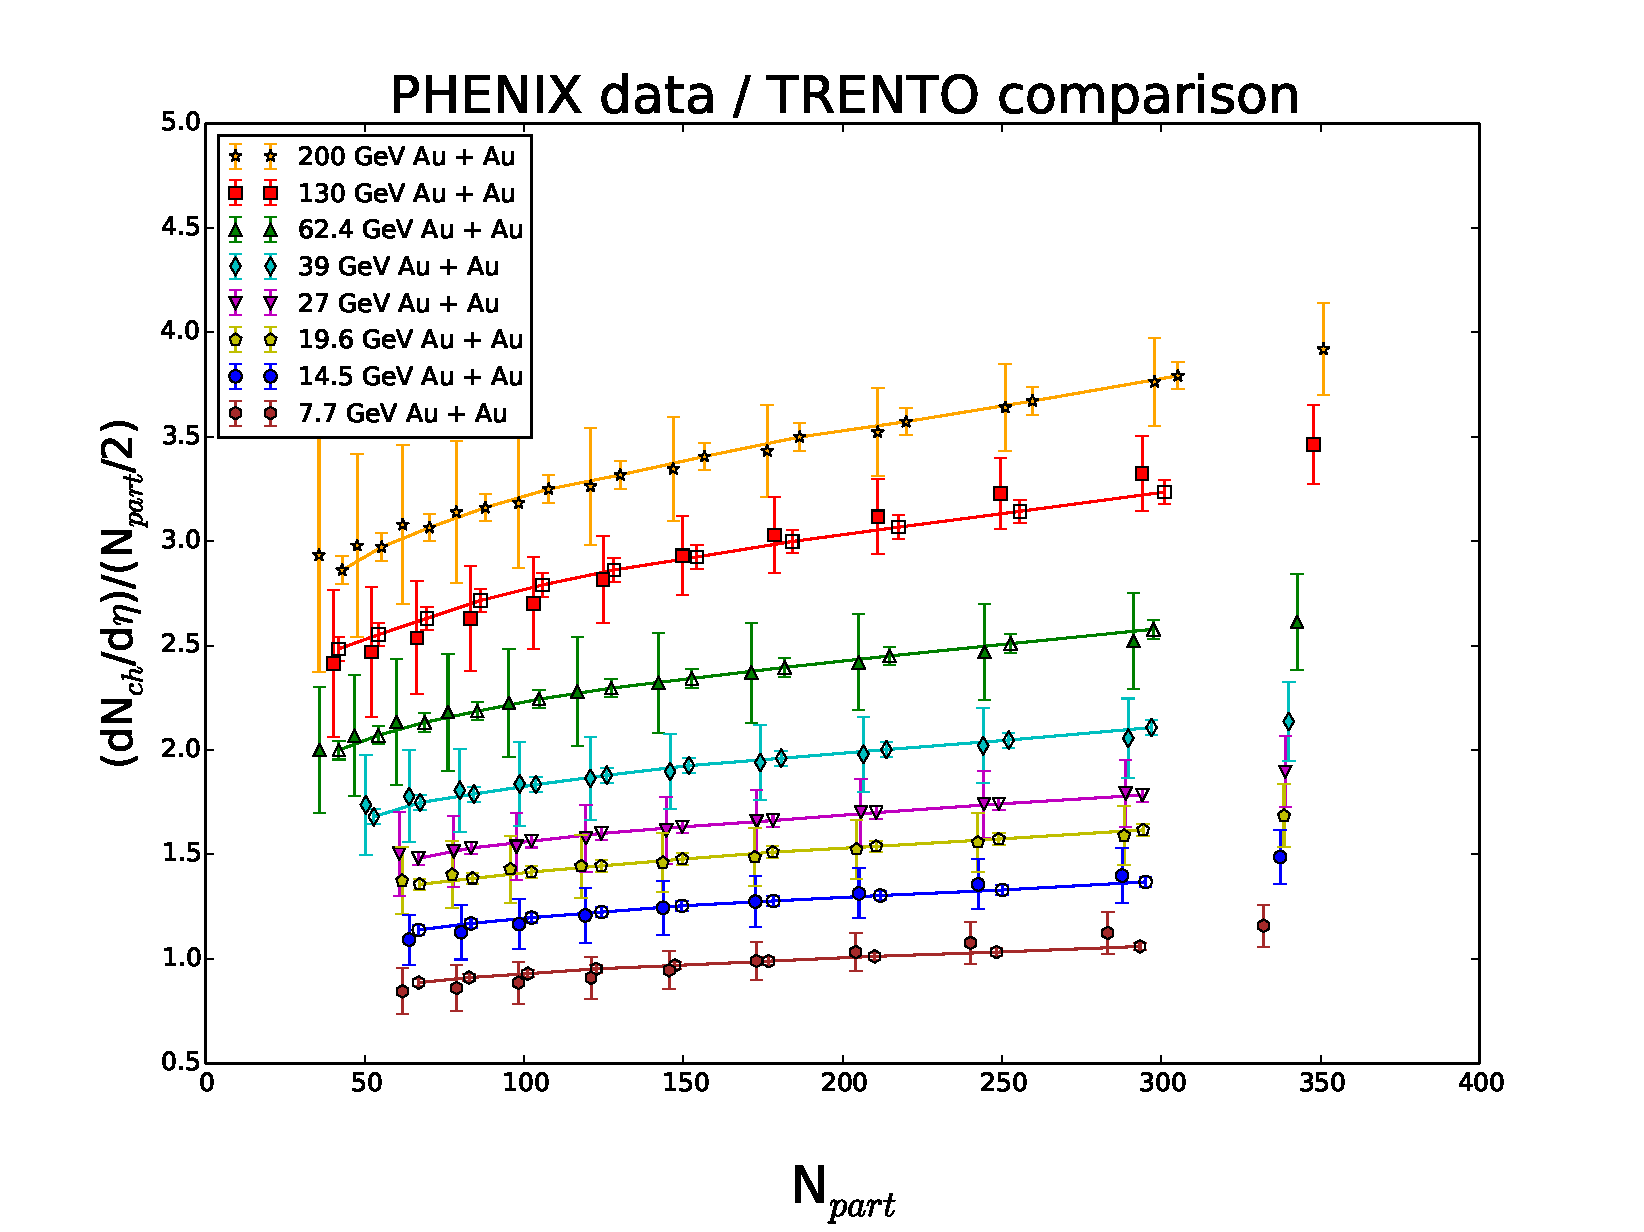
\includegraphics[width=0.8\textwidth]{phenix_trento_comp.pdf}
\label{fig_label}
\caption{Fit of \trento\ data to PHENIX data. Figure created with [python phenix\_trento\_comp.py]}
\end{center}
\end{figure}

\begin{figure}[h]
\begin{center}
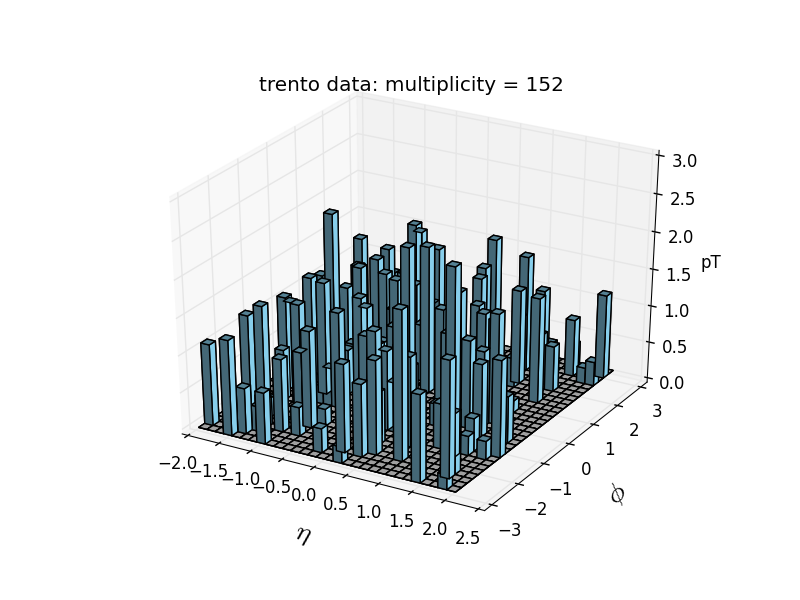
\includegraphics[width=0.49\textwidth]{2d_hist_trento.png}
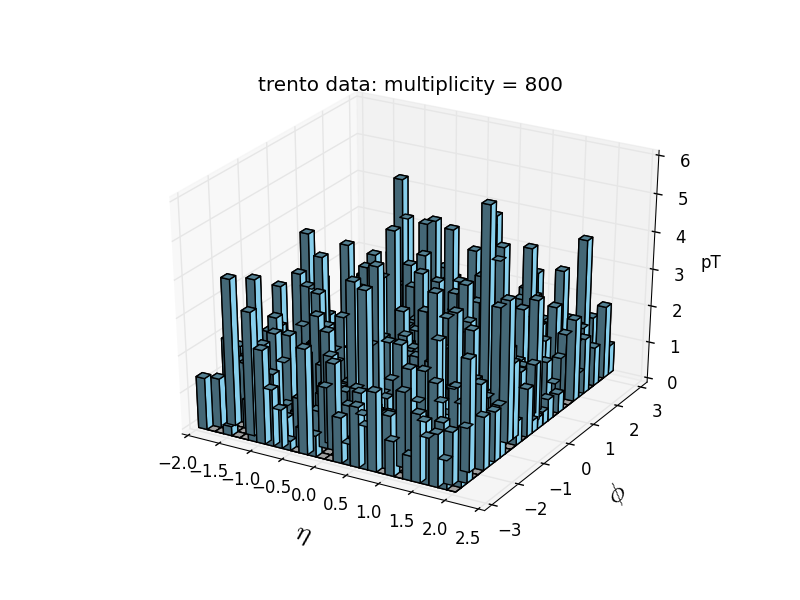
\includegraphics[width=0.49\textwidth]{2d_hist_trento2.png}
\label{fig_label}
\caption{\trento\ event display (no jets). High multiplicity is shown on the right and lower multiplicity on the left. Both plots created with [python 2d\_hist\_trento.py -b 30]}
\end{center}
\end{figure}

\section{Working with SlowJet Finder}
%
% Describe SlowJet Finder algorithm and input parameters.
% Show examples of SlowJet Finder on Pythia only.
% Show example of SlowJet Finder on Pythia plus Trento.
%
The SlowJet jet finder takes several input parameters that affect how it searches for jets. These parameters are power, radius, minimum jet $p_T$ ($p_TjetMin$), $etaMax$, select, and $massSet$. Power determines which jet finding algorithm to use. For our programs we set power to -1, this corresponds to the {\it anti-k$T$} algorithm. Other possible algorithms for SlowJet are the Cambridge/Aachen algorithm and the $kT$ algorithm. Radius is crudely related to the radius of the jet cone in ($y$,$\phi$) space. In most of our programs radius is set to 0.7 by default. $p_TjetMin$ is the minimum $p_T$ that a cluster must have to become a jet. Our values for $p_TjetMin$ are normally set to 10 or 15 GeV. $etaMax$ is the maximum +/- pseudo-rapidity that the detector is assumed to cover. For our programs $etaMax$ is always set to 2. Select determines which particles are analyzed by SlowJet. For our programs select is always set to 2 which corresponds to all observable final-state particles. $massSet$ determines the masses assumed for the particles analyzed by SlowJet. There are three $massSet$ options: 0 for all massless, 1 for photons are massless while all others are assigned the mass of charged pions, and 2 for all given their correct masses. For our programs $massSet$ is set to either 1 or 2. Radius and $p_TjetMin$ are the parameters that are most often changed while we examine jets.

Figures 5 and 6 demonstrate how well SlowJet is able to function in Pythia events with varying amounts of heavy ion background. Both figures use the same familiar event display that was shown in figures 2 and 4 and use the standard SlowJet settings discussed above. In these figures the color scheme is that Pythia jets that are identified correctly by SlowJet are colored green, particles mistakenly identified as SlowJet jets is colored yellow,  Pythia jets that are missed by SlowJet are colored red, and all other background particles are colored blue. Figure 5 shows two Pythia events with no heavy ion background. In the event shown on the left SlowJet correctly identifies both jets. However, in the event on the right, the second jet is too diffuse and SlowJet does not identify it as a jet. Figure 6 is a greater test for SlowJet because now a \trento\ background is introduced. In the low \trento\ multiplicity event, SlowJet is still able to correctly identify the two jets, however a few background particles, shown in yellow, are also lumped in with the jets.  In the high \trento\ multiplicity event SlowJet becomes confused. In this case there are many \trento\ particles identified as jets, those shown in yellow. The true jets become lost in the background and SlowJet fails.

All the bar plots in figures 5 and 6 are created in a way so that bars are stacked on top of each other if two different color bars share the same bin. The order in which the bars are stacked is that the blue bars corresponding to background not mistaken as jets goes on the bottom. The red bars associated with true jet particles not identified as jets are stacked next. Then the yellow bars associated with falsely identified jets are stacked. Correctly identified jets, shown in green, are then stacked on the very top. This order of stacking the bars is the most useful when displaying very congested events because it is easy to see how SlowJet performed.

\begin{figure}[h]
\begin{center}
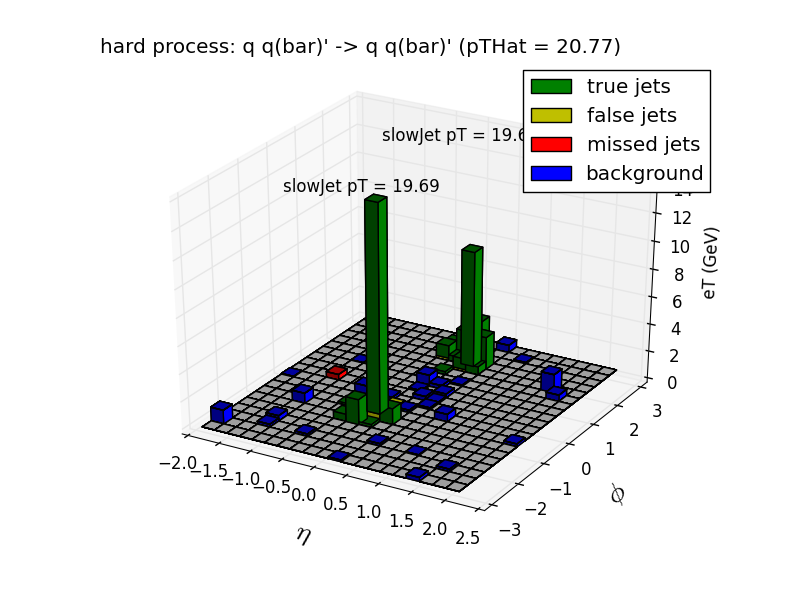
\includegraphics[width=0.49\textwidth]{2d_hist_truejet_wcol1.png}
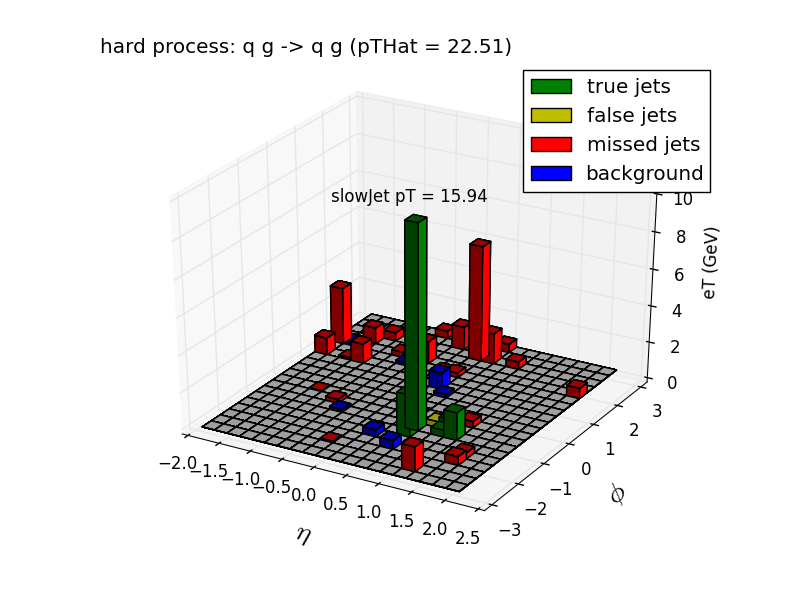
\includegraphics[width=0.49\textwidth]{2d_hist_truejet_wcol2.png}
\label{fig_label}
\caption{Event display for Pythia with SlowJet Finder, no heavy ion background.  SlowJet succeeds on the left but struggles on the right. Both plots created with [python 2d\_hist\_truejet\_wcol.py]}
\end{center}
\end{figure}

\begin{figure}[h]
\begin{center}
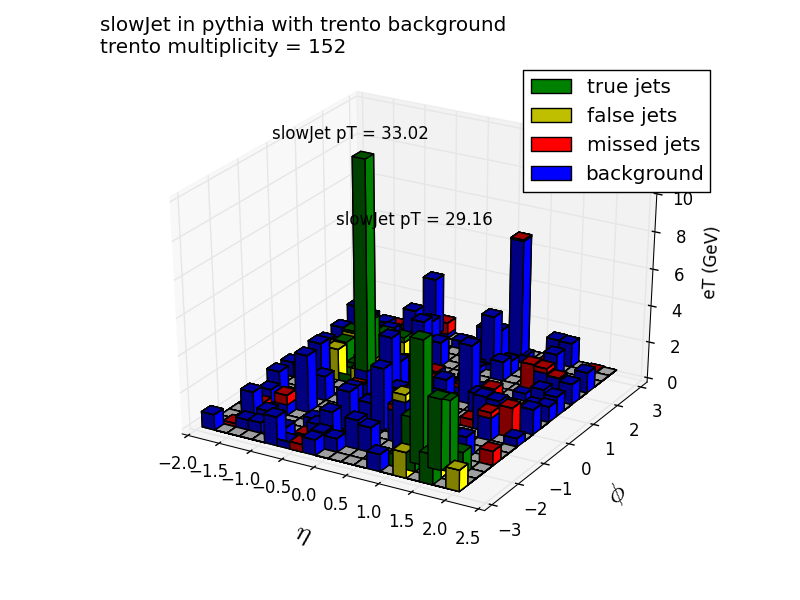
\includegraphics[width=0.49\textwidth]{truejet_wtrento1.png}
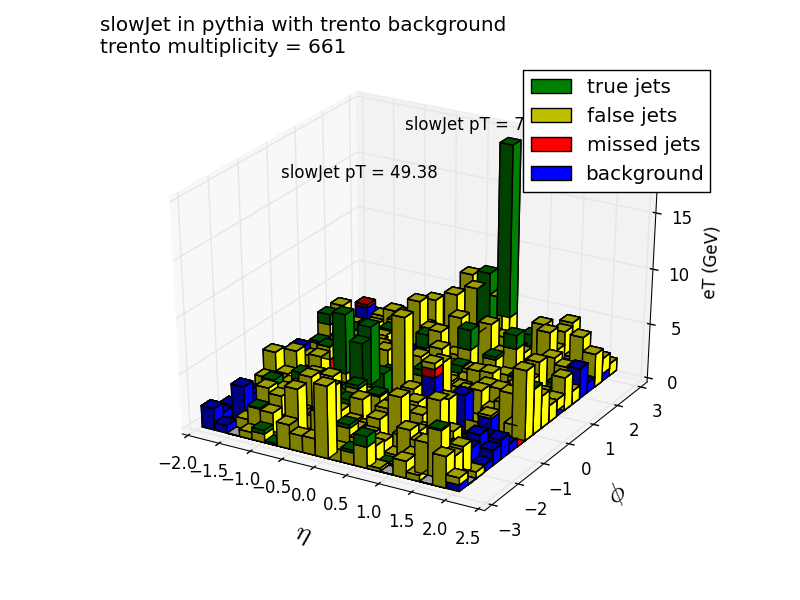
\includegraphics[width=0.49\textwidth]{truejet_wtrento2.png}
\label{fig_label}
\caption{Event display for Pythia+Trento with SlowJet Finder. Low multiplicity \trento\ background shown to the left and high multiplicity \trento\ background shown to the right. Correctly identified jets are colored green, mistakenly identified jets are colored yellow, jets that SlowJet missed are colored red, and all background particles are colored blue. Both plots created with [python truejet\_wtrento.py]}
\end{center}
\end{figure}

\section{Studying Jets}
%
% Define formula for fragmentation function.
% Explain methodology for tracing particles in jets
%
To study jets and explore the different parameters of SlowJet we first focused on the SlowJet parameters of radius and $p_TjetMin$. One of our programs examined how many jets were identified in Pythia events with \trento\ backgrounds. Ideally SlowJet should identify 2 jets for each Pythia event. We found that when $p_TjetMin$ was set low and radius was set high, far too many jets would be identified on average. However, if $p_TjetMin$ was set high and radius set low, very few jets would be identified. In the \trento\ backgrounds it is difficult to raise the requirements for clusters to be identified as jets while still being able to identify all Pythia jets. The plots produced by this program are shown in figure 7. Another program restricted the $p_T$ of Pythia jets to 20-25 GeV and set $p_TjetMin$ to 15 GeV. Radius was then varied to see if the identified jets would be in the correct $p_T$ range. We found similar results. Increasing radius to values as high as 0.8 caused the peak of identified jets to be within the proper $p_T$ range but also allowed many jets above the range to be identified as well. Decreasing radius to values as low as 0.3 caused the peak of identified jets to fall below the proper $p_T$ range but reduced the number of jets that were identified above the range.

Our next focus was on the fragmentation function value ($\xi$) for particles within both SlowJet jets and true jets. To calculate $\xi$ we used the following formula:
\[\xi = ln((\vec{p_{jet}} \cdot \vec{p_{jet}})/(\vec{p_{jet}} \cdot \vec{p_{prt}}))\]
In figure 8, $\xi$ is calculated for both QCD and QED events with no \trento\ data on the left and with \trento\ data on the right. $\xi$ is calculated for SlowJet jets with radius set at 0.3, 0.5, and 0.7 in all four plots. In the plots it is noticeable that as radius is decreased the peak of $\xi$ values for reconstructed jets is reduced. This occurs because particles with higher $\xi$ values are farther away from the center of the jet cone. As radius is decreased particles on the edge of the jet cone are no longer included in the reconstructed jets. True jets consist of all particles that are ancestors of the initial hard scattering in each Pythia event. These particles were identified by tracing the daughters of each particle starting with the two initial particles that participated in the hard process and ending when only final state particles remain.

\begin{figure}[h]
\begin{center}
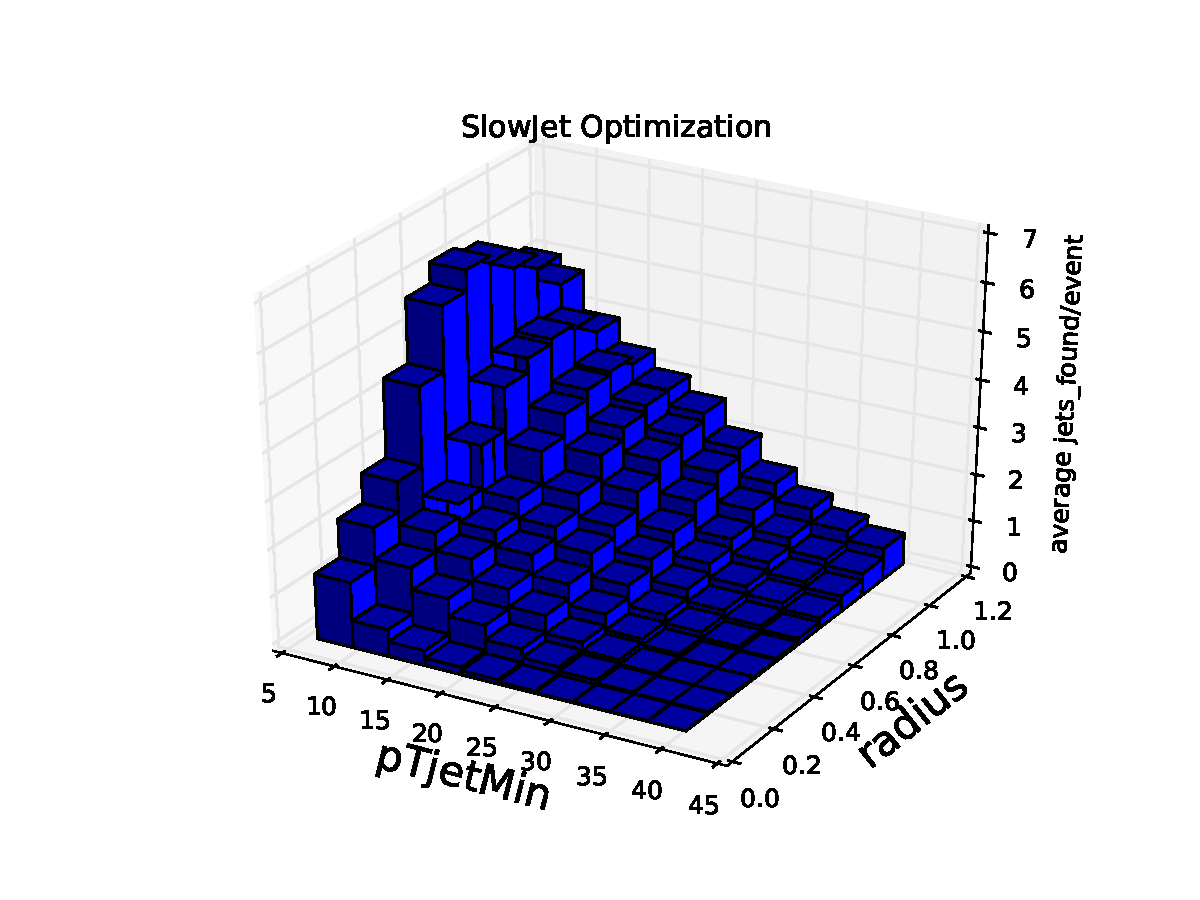
\includegraphics[width=0.49\textwidth]{optimize_slowjet1.pdf}
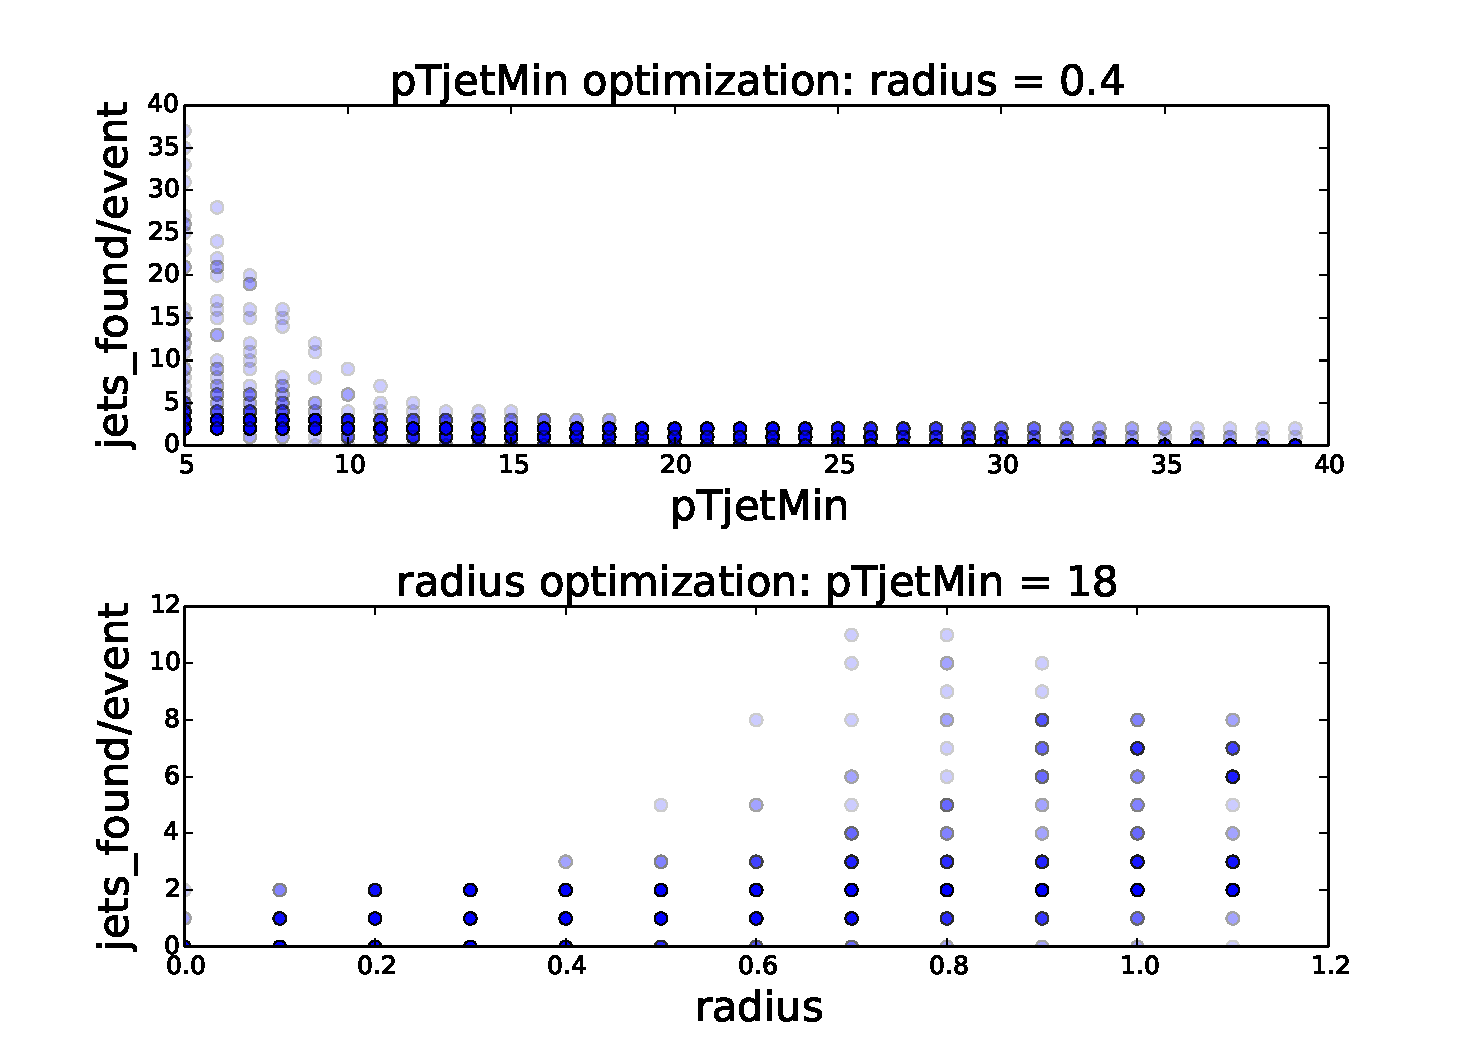
\includegraphics[width=0.49\textwidth]{optimize_slowjet2.pdf}
\label{fig_label}
\caption{The 2 dimensional histogram on the left shows the average number of jets found by SlowJet in Pythia events with \trento\ background. The plots on the right are 1 dimensional scatter plots that explore the optimization of each parameter individually. All plots created with [python optimize\_slowjet.py]}
\end{center}
\end{figure}

\begin{figure}[h]
\begin{center}
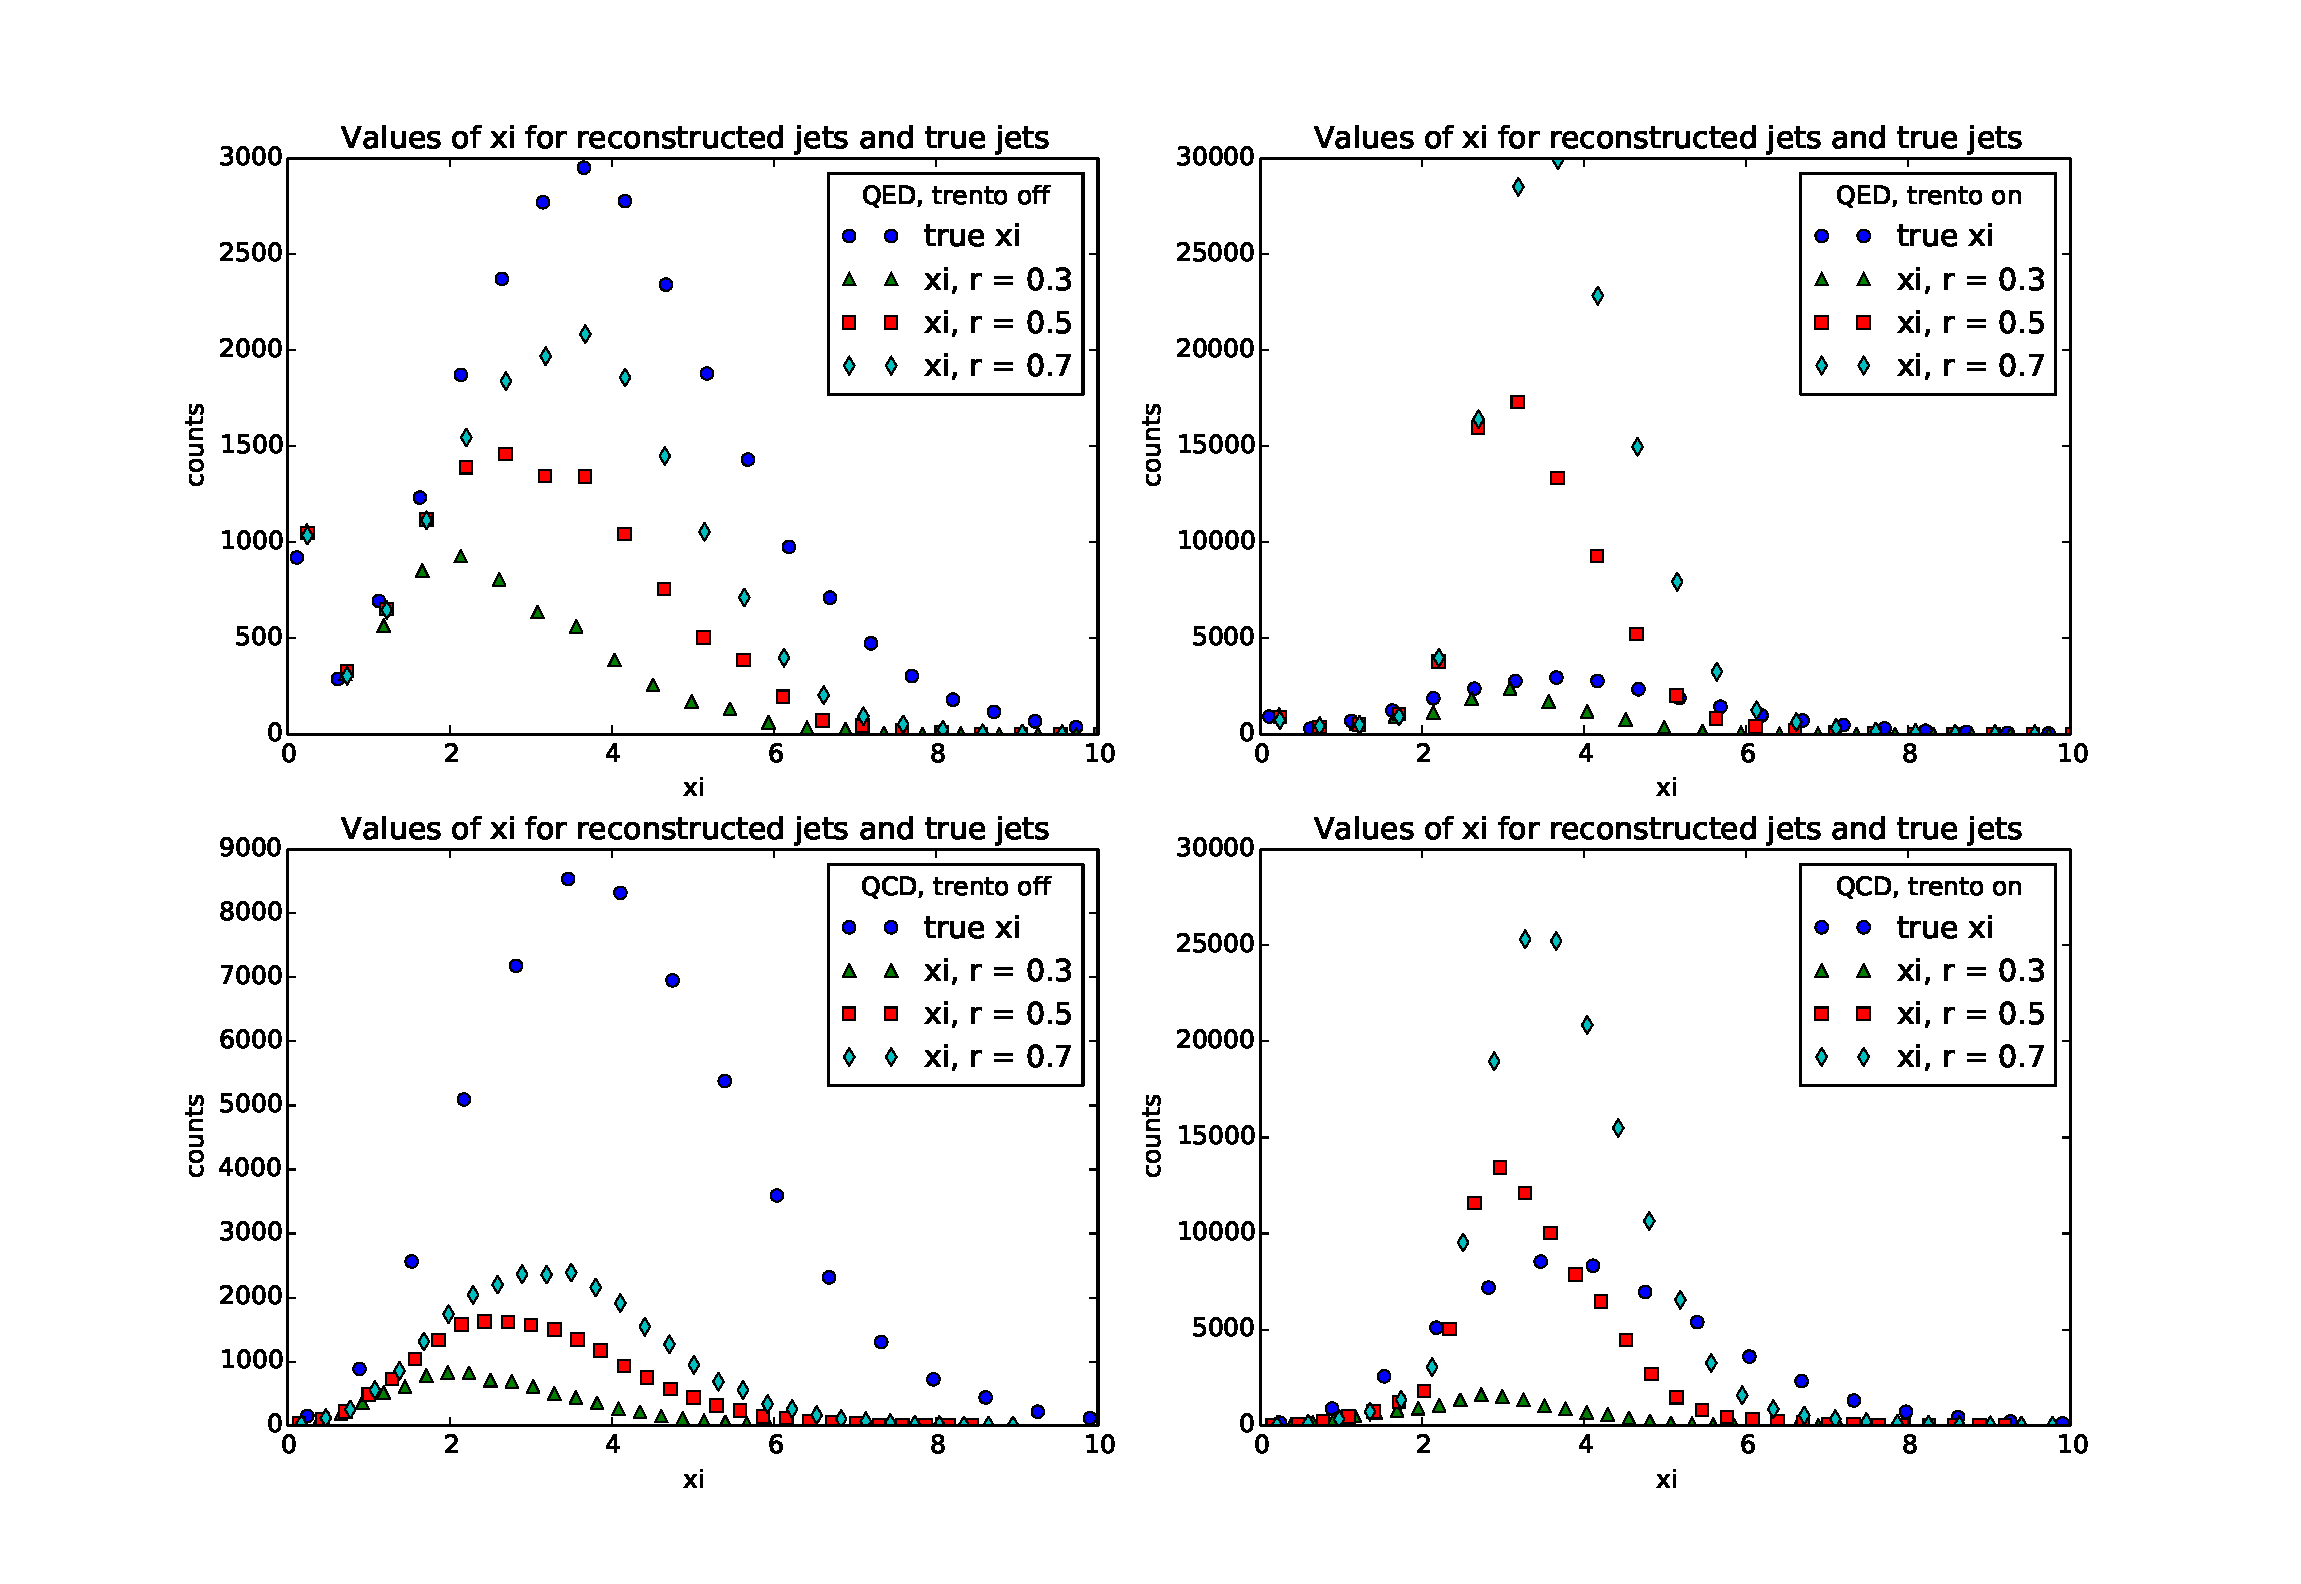
\includegraphics[width=0.9\textwidth]{compare_xi.pdf}
\label{fig_label}
\caption{Fragmentation function value ($\xi$) distributions for true and reconstructed QCD and QED jets, with and without trento backgrounds.  Figure created with [python compare\_xi.py]}
\end{center}
\end{figure}

\appendix

\section{Listing of Python Scripts}
\begin{description}
\item[2d\_hist\_jetplot\_wcol.py] Displays Pythia events in ($\eta$,$\phi$) space, SlowJet jets are colored red
\item[2d\_hist\_trento.py] Displays \trento\ backgrounds in ($\eta$,$\phi$) space
\item[2d\_hist\_truejet\_wcol.py] Displays Pythia events in ($\eta$,$\phi$) space, SlowJet jets are compared to true jets
\item[3d\_jetplot\_2016.py] Displays Pythia events in ($\eta$,$\phi$) space, particles shown individually, SlowJet jets are colored red
\item[Npart\_bins.py] Plots initial entropy (mult) vs. number of participants (Npart) for \trento\ data
\item[compare\_xi.py] Compares $\xi$ for true and reconstructed jets
\item[nCh\_pythiaEvents.py] Shows the frequency of charged multiplicities for various Pythia QCD/QED processes
\item[phenix\_data.py] PHENIX data plotted with error bars for charged multiplicity vs. number of participants, Au-Au at various energies
\item[phenix\_trento\_comp.py] Fits \trento\ data to PHENIX data for various Au-Au energies, charged multiplicity vs. number of participants
\item[phi\_pT\_eta\_trento.py] Plots the values of $\phi$, $p_T$, and $\eta$ that are created for the \trento\ backgrounds
\item[optimize\_slowjet.py] Creates a 2d histogram for SlowJet parameters radius and $p_TjetMin$ and shows average jets found for various values
\item[pT\_pythiaEvents.py] Plots frequency of various QED/QCD Pythia hard processes
\item[pythia\_slowjet\_trento\_hist.py] Displays Pythia events with \trento\ backgrounds in ($\eta$,$\phi$) space, bars are colored to show SlowJet performance
\item[restricted\_jetpT.py] Tests various values of SlowJet radius while the Pythia jets are in a restricted $p_T$ range
\item[scanPythia.py] Rrints SlowJet information about Pythia events such as jet constituents and jet $p_T$
\item[slowJetpT\_vs\_pTHat.py] Compares the true jet $p_T$ produced by Pythia QCD/QED events to the SlowJet jet $p_T$ 
\item[slowjet\_trento\_hist.py] Displays \trento\ background in ($\eta$,$\phi$) space, SlowJet identified jets are colored red
\item[trento\_in\_python.py] Creates plots for \trento\ data, such as initial entropy vs. impact parameter and number of participants vs. impact parameter, as well as others
\item[truejet\_wtrento.py] Displays Pythia events with \trento\ backgrounds in ($\eta$,$\phi$) space, SlowJet jets are compared to true jets
\item[xi\_reconstructed\_jets.py] Creates a histogram of $\xi$ values for SlowJet jets
\item[xi\_true\_jets.py] Creates a histogram of $\xi$ values for true jets
\end{description}


\end{document}